\documentclass{beamer}
\usepackage{beamerthemesplit}
\usepackage{amsmath}
\usepackage{amssymb}
\usepackage{pause}
\usepackage{subfigure}
%\usepackage{subfig}
\usepackage{amsfonts}
\usepackage{newlfont}
\usepackage{graphics}
\usepackage{graphicx}
\usepackage{epsfig}
\usepackage[latin1]{inputenc}
\usepackage{hyperref}
\usepackage[numbers,square]{natbib}
%\usepackage[round]{natbib}
\usepackage[english]{babel}
% \usetheme{default}
% \usetheme{Boadilla} %# not so good
% \usetheme{Madrid}  % # not so good
% \usetheme{Montpellier}
 %\usetheme{Warsaw}
% \usetheme{Copenhagen}
% \usetheme{Goettingen}
% \usetheme{Hannover}
\usetheme{Berkeley}
\usecolortheme{crane}
\beamertemplatesolidbackgroundcolor{white!25}
\setlength{\parskip}{8pt plus 1pt minus 1pt}
\setbeamertemplate{footline}[frame number]
\title[ABV-IIITM Gwalior]{ANALYSIS OF MALICIOUS CODE DYNAMICS WITH TARGET AND ATTACKER NODES USING MATHEMATICAL MODEL}
\author{Alok Singh (2014IPG-009)\\
Neha Singh (2014IPG-059)\\
Saurabh Sharma (2014IPG-078)}
\tiny \institute[]{
ATAL BIHARI VAJPAYEE INDIAN INSTITUTE OF INFORMATION TECHNOLOGY AND
MANAGEMENT\\
20-09-2017\\
\begin{figure}[h]

\includegraphics[width=0.80cm]{iiitm}
\end{figure}
}
%\date{\today}
\begin{document}
\frame{\titlepage}


\begin{frame}\frametitle{Contents}
\begin{itemize}
\item Introduction
\item Literature Review
\item Problem Statement and Objective
\item Schematic Flow of Proposed Compartmental Model
\item Numerical Experimentation (Feasibility States)
\item Numerical Experimentation (No Security)
\item Analysis of media coverage factor
\item Analysis of Sensitivity
\item Conclusion and Future Scope
\item References
\end{itemize}
\end{frame}

\begin{frame}\frametitle{\section{Introduction}Introduction}
\begin{itemize}
\item Malicious code is any code intentionally integrated, converted or cut out from a
software system to damage or debase the system's predetermined function, e.g., Virus, Worms, Ransom-Ware.
\item Propagation of malicious codes is epidemic in nature.
\item To predict the behavior of cyber threats and to make the secure cyber system, it is necessary to
study and find out the different types of malicious objects.
\end{itemize}
\end{frame}


\begin{frame}\frametitle{\section{Literature Review}Literature Review}
\begin{table}
\label{table:sen1}
\begin{tabular}{|p{1.5 cm}|p{3 cm}|p{2 cm}|p{2.5 cm}|}
\hline
\bf Author & \bf Paper Title &\bf Publishing Details &\bf Salient Features\\
\hline
A. K. Misra,M. Verma and A. Sharma&Capturing the interplay between malware and anti-malware in a computer network &Applied Mathematics and Computation 2014 &Effect of antivirus over a system \cite{edtr5}\\
\hline
\end{tabular}
\end{table}
\end{frame}

\begin{frame}\frametitle{Literature Review}
\begin{table}
\label{table:sen}
\begin{tabular}{|p{1.5 cm}|p{3 cm}|p{2 cm}|p{2.5 cm}|}
\hline
\bf Author & \bf Paper Title &\bf Publishing Details &\bf Salient Features\\
\hline
Bhargava, D.Soni, P.jain, J.Dhar&Dynamics of attack of malicious codes on the targeted network &ICRTIT, IEEE 2016&Malicious code dynamics and effect of firewall\cite{edtr15} \\
\hline
G. P. Sahu,J. Dhar&SEIQHRS epidemic model with media coverage, quarantine and isolation in a community with pre-existing immunity&J. Mathematical Analysis and Applications, Elsevier 2015&An epidemic model SEQIHRS is proposed with quarantine and isolation control strategies \cite{edtr13}\\
\hline

\end{tabular}
\end{table}
\end{frame}

\begin{frame}\frametitle{Literature Review}
\begin{table}
\label{table:sen2}
\begin{tabular}{|p{1.5 cm}|p{3 cm}|p{2 cm}|p{2.5 cm}|}
\hline
\bf Author & \bf Paper Title &\bf Publishing Details &\bf Salient Features\\
\hline
A. Grey et. al.&A stochastic differential equation SIS epidemic model & SIAM J. Applied Mathematics 2011&Analysis of stochastic  SIS model \cite{edtr17}\\
\hline
Kribs-Zaleta and Velasco-Hernandez& A simple vaccination model with multiple endemic states & Mathematical biosciences 2002 & Effect of vaccination on basic reproduction number for a large population \cite{edtr21}\\
\hline
\end{tabular}
\end{table}
\end{frame}

\begin{frame}\frametitle{\section{Problem Statement and Objective}Problem Statement and Objective}
The objective of this project is to analyze the malicious code dynamics with the target
and attacker nodes using a mathematical model.
\end{frame}


\begin{frame}\frametitle{\section{Proposed Model}Schematic Flow of Proposed Compartmental Model}
\begin{figure}[h]
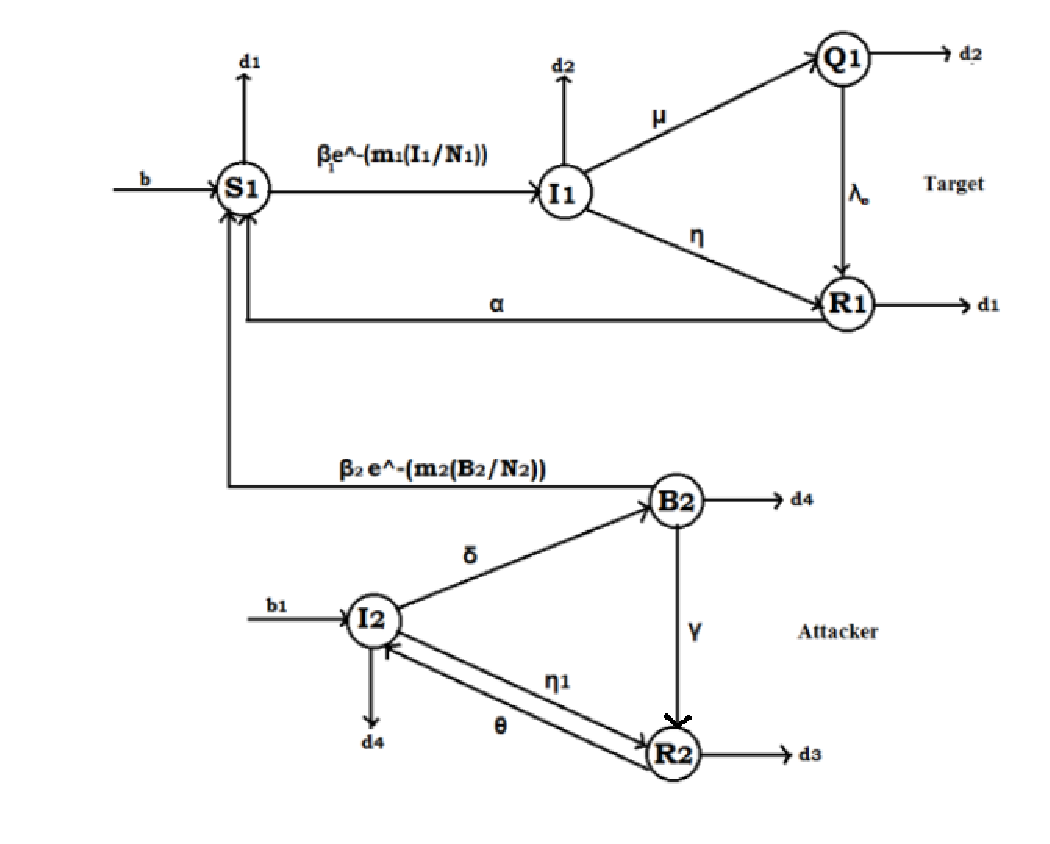
\includegraphics[width=4.0in]{13-DR1}

\caption{Schematic Flow of the Compartmental Model}
\label{13-DR1}
\end{figure}
\end{frame}

\begin{frame}\frametitle{{Parameters Descriptions}}
\tiny \begin{table}
\begin{tabular}{|p{2 cm}|p{7 cm}|}
\hline
\bf Parameters & \bf Description \\
\hline
b, $b_1$ & Recruitment rates of target and attacker classes\\
\hline
$d_1$, $d_3$ & Natural death rate of targeted and attacker population node\\
\hline
$\beta_1$ & Contact rate from susceptible class to infected class\\
\hline
$\beta_2$ & Contact rate from breaking-out to susceptible class\\
\hline
$\gamma$ &Rate of recovery of computers with malicious codes in breaking-out state\\
\hline
$\eta$, $\eta_1$ &Rate of recovery of computers with malicious codes in infected state\\
\hline
$d_2$ &Death rate in infected target classes(death due to infection and natural death)\\
\hline
$\lambda_0$ &Rate of recovery of computers with malicious codes in quarantine state\\
\hline
$\delta$ &Rate of change of malicious nodes from infected to breaking-out state\\
\hline
$\theta$ &Rate of change of recovered nodes into infected nodes\\
\hline
$d_4$ &Death rate in infected attacker classes(death due to infection and natural death)\\
\hline
$\alpha$ &Rate of change of recovered nodes into susceptible nodes\\
\hline
$m_1$, $m_2$ &Infection controlling coefficients\\
\hline
$\mu$ &Rate of change of malicious nodes from infected to quarantine state\\
\hline
\end{tabular}
\caption {Description of Parameters}
\label{table:param1a}
\end{table}
\end{frame}

\begin{frame}\frametitle{Proposed mathematical model}
{\bf For targeted nodes:}
{\footnotesize \begin{eqnarray*}
% \nonumber % Remove numbering (before each equation)
  \frac{d \tilde S_1}{d \tilde t}  &=&  b-d_1 \tilde S_1+ \tilde \alpha \tilde R_1 - \tilde \beta_1 e^{-m_1 \left(\frac{ \tilde I_1}{ \tilde N_1}\right)}\left(\frac{ \tilde I_1}{ \tilde N_1}\right) \tilde S_1- \tilde \beta_2 e^{-m_2 \left(\frac{ \tilde B_2}{ \tilde N_2}\right)} \left(\frac{ \tilde B_2}{ \tilde N_2}\right) \tilde S_1\\
   \frac{d \tilde I_1}{d \tilde t} &=& \tilde \beta_1 e^{-m_1 \left(\frac{\tilde I_1}{\tilde N_1}\right)}\left(\frac{\tilde I_1}{\tilde N_1}\right) \tilde S_1+\tilde \beta_2 e^{-m_2 \left(\frac{\tilde B_2}{\tilde N_2}\right)} \left(\frac{\tilde B_2}{\tilde N_2}\right)\tilde S_1 - (\tilde d_2+ \tilde\eta +\tilde \mu)\tilde I_1 \\
  \frac{d \tilde Q_1}{d \tilde t} &=& \tilde \mu \tilde I_1 -\tilde d_2 \tilde Q_1 - \tilde \lambda_0 \tilde Q_1 \\
 \frac{d \tilde R_1}{d \tilde t} &=&  \tilde\lambda_0 \tilde Q_1-\tilde \alpha \tilde R_1-d_1 \tilde R_1+ \tilde\eta \tilde I_1
\end{eqnarray*}}

{\bf For attacker nodes:}
{\footnotesize \begin{eqnarray*}
% \nonumber % Remove numbering (before each equation)
 \frac{d \tilde I_2}{d \tilde t} &=& b_1- \tilde d_4 \tilde I_2-\tilde \delta \tilde I_2 +\tilde \theta \tilde R_2 -\tilde\eta_1 \tilde I_2 \\
 \frac{d \tilde B_2}{d \tilde t} &=& \tilde\delta\tilde I_2 -\tilde d_4 \tilde B_2 -\tilde\gamma\tilde B_2 \\
\frac{d \tilde R_2}{d \tilde t} &=& \tilde\gamma \tilde B_2 - d_3 \tilde R_2 - \tilde \theta\tilde R_2+\tilde \eta_1\tilde I_2
\end{eqnarray*}}
\end{frame}

\begin{frame}\frametitle{\section{Analysis}Boundedness of the system}
\begin{itemize}
\item For targeted population,
\begin{equation*}\Omega_k = \{( \tilde S_1, \tilde I_1, \tilde Q_1, \tilde R_1) \in R_+ \textsuperscript{4} : \tilde S_1+ \tilde I_1 + \tilde Q_1 + \tilde R_1 \leq b/d  \}\end{equation*}
And for Attacker population
\begin{equation*}\Omega_{k1} = \{( \tilde I_2, \tilde B_2, \tilde R_2) \in R_+ \textsuperscript{3} : \tilde I_2 + \tilde B_2 + \tilde R_2 \leq b_1/d_1  \}\end{equation*}
\item Steady States and their Stability : Two equilibrium states are
observed out of which one is malicious-codes free and another is
endemic equilibrium states.
\end{itemize}
\end{frame}

\begin{frame}\frametitle{Proposed mathematical model(Non- Dimensional)}
Due to complicated nature of the equations, the equations are non-dimensionalized for the above system using:
\small
\begin{equation*}
S_1=\frac{ \tilde S_1}{ \tilde N_1}, \hspace{0.5 cm} I_1=\frac{ \tilde I_1}{ \tilde N_1}, \hspace{0.5 cm} Q_1=\frac{ \tilde Q_1}{ \tilde N_1} \hspace{0.5 cm}
R_1=\frac{ \tilde R_1}{\tilde N_1},\end{equation*}
\small \begin{equation*}I_2=\frac{ \tilde I_2}{\tilde N_2},  \hspace{0.5 cm} B_2=\frac{\tilde B_2}{\tilde N_2},  \hspace{0.5 cm} R_2=\frac{\tilde R_2}{\tilde N_2}, \hspace{0.5 cm} t=\tilde d_1 \tilde t,\end{equation*}
\small\begin{equation*} N_1=\frac{\tilde N_1}{ \tilde N_1\textsuperscript{0}},  \hspace{0.5 cm} N_2=\frac{\tilde N_2}{ \tilde N_2\textsuperscript{0}},  \hspace{0.5 cm} \tilde N_1\textsuperscript{0}=\frac{b}{\tilde d_1},  \hspace{0.5 cm} \tilde N_2\textsuperscript{0}=\frac{b_1}{\tilde d_3}
\end{equation*}
\end{frame}

\begin{frame}\frametitle{Proposed mathematical model(Non-Dimensional)}
{\bf For targeted nodes:}
\tiny \begin{eqnarray*}
\frac{d S_1}{dt} &=& \frac{( 1- S_1)}{N_1}+ \alpha R_1 - \beta_1 e^{-m_1 I_1} I_1 S_1- \beta_2 e^{-m_2 B_2} B_2 S_1-S_1+S_1^2 \nonumber \\
&+& d_2 I_1 S_1+d_2 Q_1 S_1+R_1 S_1
\end{eqnarray*}
\tiny \begin{eqnarray*}
\frac{d I_1}{dt}&=& \beta_1 e^{-m_1 I_1} I_1 S_1 +\beta_2 e^{-m_2 B_2} B_2 S_1 - ( d_2+ \eta + \mu) I_1- \frac{ I_1}{N_1}+d_2 I_1^2 \nonumber\\
&+& I_1 S_1+d_2 Q_1 I_1+I_1 R_1
\end{eqnarray*}
\tiny \begin{equation*}
\frac{d Q_1}{dt}= \mu I_1 - d_2 Q_1 - \lambda_0 Q_1- \frac{ Q_1}{N_1}+d_2 Q_1^2+d_2 I_1 Q_1+ Q_1 S_1+Q_1 R_1
\end{equation*}
\tiny \begin{equation*}
\frac{d R_1}{dt}=\lambda_0 Q_1- \alpha R_1- R_1+ \eta I_1- \frac{ R_1}{N_1}+R_1^2+d_2 I_1 R_1+d_2 Q_1 R_1+R_1 S_1
\end{equation*}

{\bf For attacker nodes:}
\tiny \begin{eqnarray*}
% \nonumber % Remove numbering (before each equation)
  \frac{d I_2}{dt }&=&  \frac{( 1- I_2)}{N_2}- d_4 I_2-\delta I_2 + \theta R_2 -\eta_1 I_2+ d_4 I_2^2+d_4 I_2 B_2+ I_2 R_2 \\
 \frac{d B_2}{d t}&=& \delta I_2 - d_4 B_2 -\gamma B_2- \frac{ B_2}{N_2}+d_4 B_2^2+d_4 I_2 B_2+ B_2 R_2  \\
   \frac{d R_2}{d t} &=& \gamma B_2 - R_2 - \theta R_2+ \eta_1 I_2- \frac{ R_2}{N_2}+R_2^2+d_4 I_2 R_2+d_4 B_2 R_2
\end{eqnarray*}
\end{frame}


\begin{frame}\frametitle{Basic Reproduction Number}
 Basic Reproduction Number : It is defined by the expected number of secondary cases
produced by a single infection in a completely susceptible population..

\par Observed basic reproduction number for this model is calculated
by using \mathcal F and \mathcal V matrices with the infectious nodes (I_1, Q_1, I_2, B_2),\\
{\footnotesize\[
\mathcal F=
\begin{bmatrix}
\beta_1 e^{-m_1 I_1} I_1 S_1- \beta_2 e^{-m_2 B_2} B_2 N_2 S_1 \\
Q_1 S_1 \\
0 \\
0
\end{bmatrix}
\]}
{\footnotesize\[
\mathcal V=
\begin{bmatrix}
( d_2+ \eta + \mu) I_1+ \frac{ I_1}{N_1}-d_2 I_1^2- I_1 S_1-d_2 Q_1 I_1-I_1 R_1\\
- \mu I_1 + d_2 Q_1 + \lambda_0 Q_1+ \frac{ Q_1}{N_1}-d_2 Q_1^2-d_2 I_1 Q_1-Q_1 R_1\\
- \frac{( 1- I_2)}{N_2}+ d_4 I_2+\delta I_2 - \theta R_2 +\eta_1 I_2- d_4 I_2^2-d_4 I_2 B_2- I_2 R_2\\
-\delta I_2 + d_4 B_2 +\gamma B_2+ \frac{ B_2}{N_2}-d_4 B_2^2-d_4 I_2 B_2- B_2 R_2
\end{bmatrix}
\]}
\end{frame}

\begin{frame}\frametitle{Contd..}
 Now, calculating Jacobian of $\mathcal F$ and $\mathcal V$ as F and V respectively,\\
F=
{\footnotesize\[
\begin{bmatrix}
(\beta_1+1) S_1 & 0 & 0 & \beta_2 S_1 \\
0 & S_1 & 0 & 0 \\
0 & 0 & 0 & 0 \\
0 & 0 & 0 & 0
\end{bmatrix}
\]}
V=
{\footnotesize\[
\begin{bmatrix}
( d_2+ \eta + \mu+1) & 0 & 0 & 0 \\
-\mu & (d_2+\lambda_0+1) & 0 & 0 \\
0 & 0 & (1+d_4+\delta+\eta_1) & 0 \\
0 & 0 & -\delta & (d_4+\gamma+1)
\end{bmatrix}
\]}
\par  Then, the dominant eigenvalue of FV\textsuperscript{-1}
is the basic reproduction number $R_{0}$.
\begin{equation*} R_0 = max \{\frac{(\beta_1+1) S_1}{(d_2+\mu+\eta+1)},\frac{S_1}{(d_2+\lambda_0+1)} \} \end{equation*}
\end{frame}

\begin{frame}\frametitle{Dynamic Behavior and Results}
Malicious-code free equilibrium $E_1$ is stable if the reproduction number $R_0$\textless1.
Endemic equilibrium $E_2$ is stable if $R_0$$>$1.

\end{frame}
\begin{frame}\frametitle{Dynamic Behavior and Results}
The local stability of malicious codes
free and endemic equilibrium is verified by the eigenvalues of the
variational matrix. If all the eigenvalues have negative real part,
then the equilibrium point is said to be asymptotically stable.
\small
\[
J=
\begin{bmatrix}
-2+2 S_1&a_{12}&d_2 S_1&\alpha+S_1&0&-\beta_2 S_1&0\\
0&a_{22}&0&0&0&\beta_2 S_1&0\\
0&\mu&a_{33}&0&0&0&0\\
0&\eta&\lambda_0&a_{44}&0&0&0\\
0&0&0&0&a_{55}&0&\theta\\
0&0&0&0&\delta&-1-d_4-\gamma&0\\
0&0&0&0&\eta_1&\gamma&-2-\theta\\
\end{bmatrix}
\]
Where,
{\footnotesize \begin{eqnarray*}
a_{12}&=& d_2 S_1-\beta_1 S_1\\
a_{22}&=&-1-d_2-\eta-\mu+\beta_1 S_1+S_1 \\
a_{33}&=&-1-d_2-\lambda_0+S_1 \\
a_{44}&=&-2+\alpha+S_1\\
a_{55}&=&-1-d_4-\eta_1-\delta
\end{eqnarray*}}
\end{frame}

\begin{frame}\frametitle{Numerical Experimentation (Feasible States)}
Possible steady states with respect to the reproduction number for different parameter
set(Dimensional and non-dimensional) in the model.
\tiny \begin{table}[h]

\label{table:feas}
\begin{tabular}{|p{2.5 cm}|l|l|p{2.5 cm}|l|l|}
\hline
\bf Parameters (Non-Dimensional) & \bf Set A& \bf Set B& \bf Parameters (With Dimensions)& \bf Set C& \bf Set D \\
\hline
b &7.5&7.5&b&1&75\\
$d_1$ &0.003&0.003&$d_1$&0.3&0.3\\
$\beta_1$ &0.001&0.01&$\tilde \beta_1$&0.5&2.5\\
$\beta_2$ &0.006&0.30&$\tilde\beta_2$&0.6&0.6\\
$\mu$ &0.003&0.003&$\tilde\mu$ &0.3&0.3\\
$\lambda_0$ &0.008&0.0008&$\tilde\lambda_0$&0.8&0.8\\
$d_4$ &0.075&0.0075&$\tilde d_4$&10&2.5\\
$b_1$ &7.5&7.5&$\tilde b_1$ &75&75\\
$d_3$ &0.02&0.02&$\tilde d_3$&2.0&2.0\\
$\eta$ &0.004&0.0004&$\tilde\eta$ &0.4&0.4\\
$\eta_1$ &0.175&0.0175&$\tilde\eta_1$&17.5&7.5\\
$\alpha$ &0.010&0.0005&$\tilde\alpha$&1.0&1.0\\
$d_2$ &0.4&0.004&$\tilde d_2$&0.4&0.4\\
$\gamma$ &0.0005&0.01&$\tilde\gamma$ &0.75&0.75\\
$\delta$&0.009&0.027&$\tilde\delta$&1.9&0.9\\
$\theta$ &0.10&0.20&$\tilde\theta$&10&10\\
$m_1$ &2&2&$m_1$&6&2\\
$m_2$ &3&2&$m_2$&6&2\\
\hline
Feasible SS&$E_1$&$E_2$&Feasible SS&$E_1$&$E_2$\\
\hline
$R_{01}$&0.0098&1.2500&&&\\
$R_{02}$&0.0073&0.3846&$\tilde R_{0}$&0.4545&2.2727\\
\hline
\end{tabular}
\end{table}
\end{frame}

\begin{frame}\frametitle{Simulation}

\begin{figure}
  \centering
  \subfloat \label{fig:a}{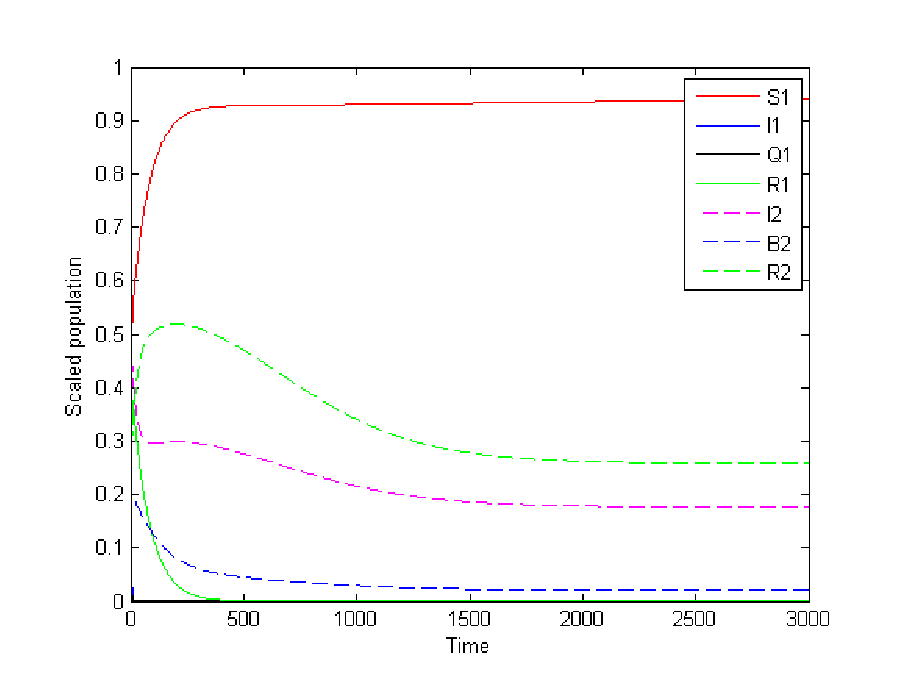
\includegraphics[height=6cm,width=4.5cm]{13-DR3}}\qquad
  \subfloat \label{fig:b}{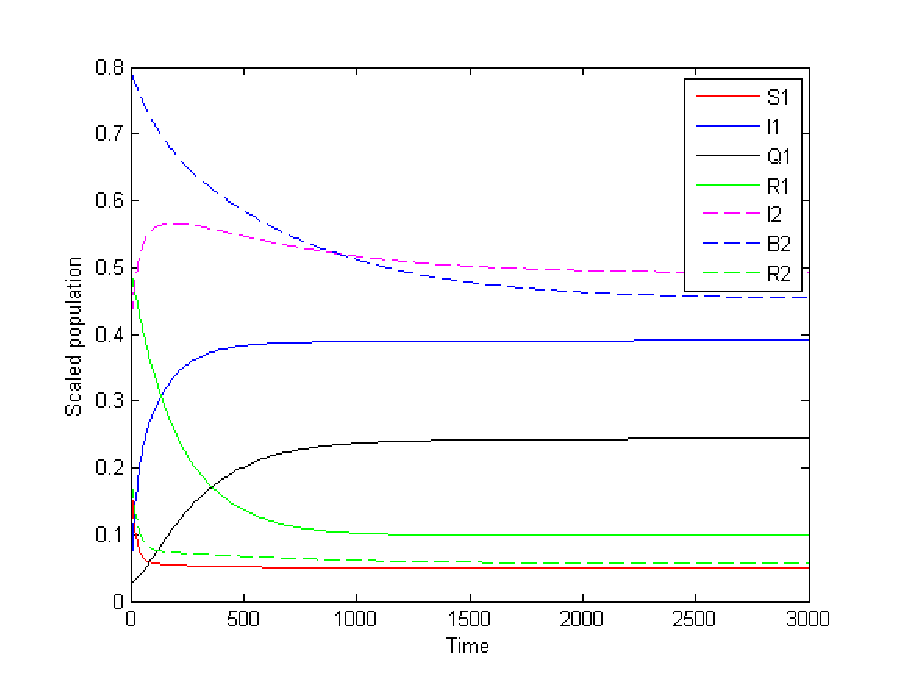
\includegraphics[height=6cm,width=4.5cm]{13-DR8}}
\caption{Node density vs Time for set A (left) and set B (right)}
\label{fig:1}
\end{figure}
\end{frame}



\begin{frame}\frametitle{Numerical Experimentation(No Security)}
\begin{figure}
  \centering
  \subfloat \label{fig:c}{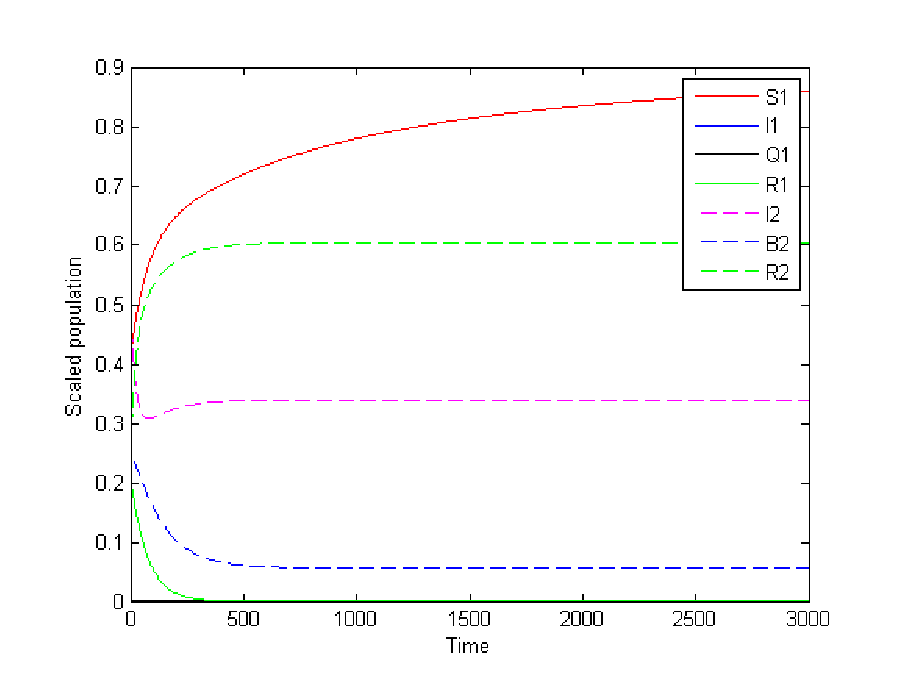
\includegraphics[height=6cm,width=4.5cm]{13-DR10}}\qquad
  \subfloat \label{fig:d}{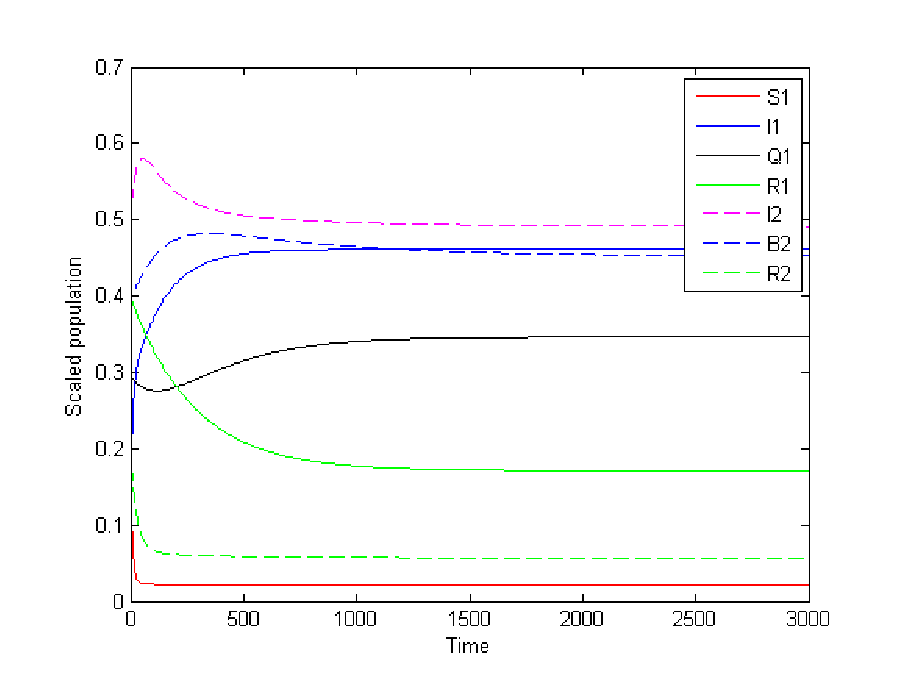
\includegraphics[height=6cm,width=4.5cm]{13-DR15}}
\caption{Node density vs Time for set A (left) and set B(right)}
\label{fig:2a}
\end{figure}

\end{frame}


\begin{frame}\frametitle{Analysis of firewall coverage}
\begin{figure}
  \centering
  \subfloat \label{fig:e}{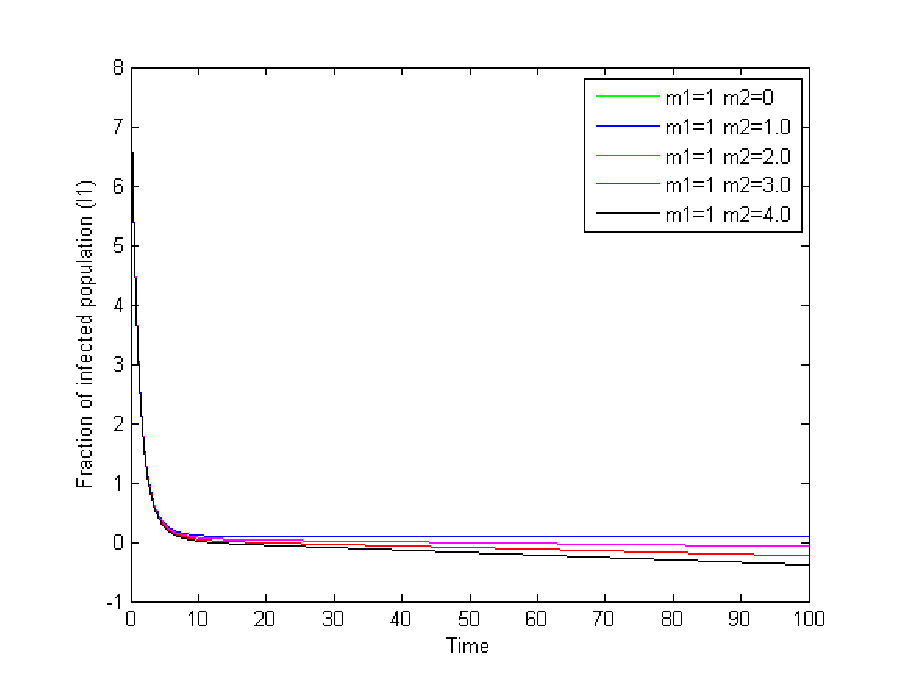
\includegraphics[height=6cm,width=4.5cm]{13-DR11}}\qquad
  \subfloat \label{fig:f}{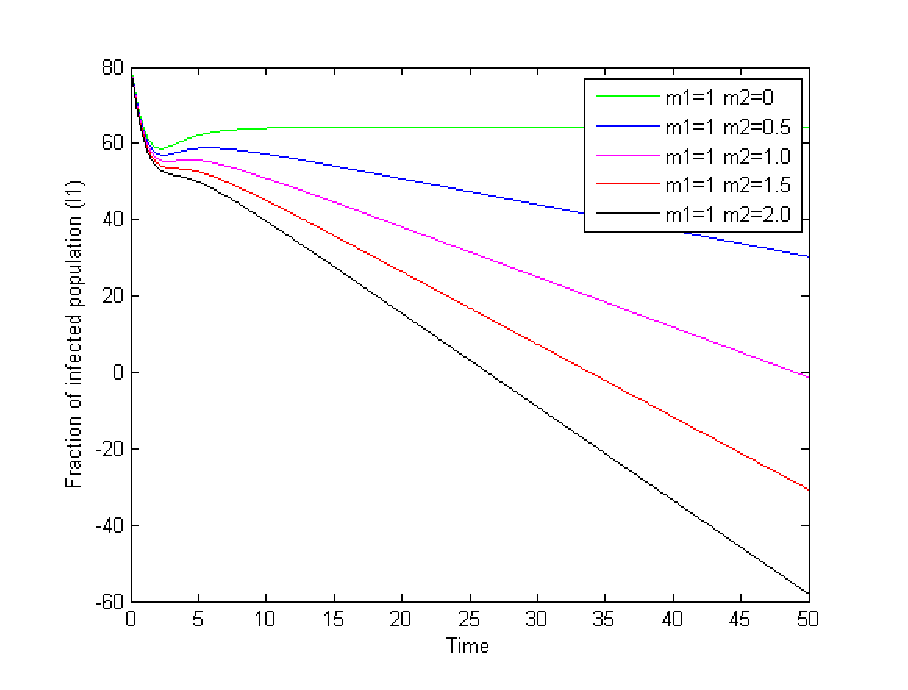
\includegraphics[height=6cm,width=4.5cm]{13-DR12}}
\caption{ Effect of $m_2$ (firewall coefficient) on $ \tilde I_1$ when $\tilde R_0 < 1$ (left) and $\tilde R_0 > 1$(right)}
\label{fig:2b}
\end{figure}

\end{frame}


\begin{frame}\frametitle{Sensitivity analysis of the system parameters}
\begin{itemize}
\item Sensitivity indices enables us
to measure the relative change in a state variable with respect to a
small change in the system parameter \cite{edtr14}.
\item Estimation and measurement of highly sensitive parameter should
be done carefully, because a small change in the parameter will lead to
relatively huge quantitative change.
\item With respect to each parameter, we derived analytical expressions
for sensitivity index of the most significant reproduction number $R_{01}$. We observed most sensitive parameters for
Basic Reproduction Numbers which are shown in the table.
\end{itemize}
\end{frame}

\begin{frame}\frametitle{Sensitivity Analysis}
\tiny {\begin{table}[h]
\label{table:sens}
\begin{tabular}{|p{2 cm}|p{2 cm}|p{2 cm}|p{2 cm}|}
\hline
\bf Parameters ($y_j$) & \bf Sensitivity $ \Upsilon_{y_j}^{R_{01}} $&\bf $ \Upsilon_{y_j}^{R_{01}} $ Set 1&\bf $ \Upsilon_{y_j}^{R_{01}} $ Set 2 \\
\hline
b &0&0&0\\
$d_1$ &0&0&0\\
$\beta_1$ &$\frac{\beta_1}{\beta_1 +1}$&0.000999&0.0099\\
$\beta_2$ &0&0&0\\
$\mu$ &$-\frac{\mu}{d_2+\mu+\eta+1}$&-0.002&-0.00298\\
$\lambda_0$ &0&0&0\\
$d_4$ &0&0&0\\
$b_1$ &0&0&0\\
$d_3$ &0&0&0\\
$\eta$ &$-\frac{\eta}{d_2+\mu+\eta+1}$&-0.0028&-0.000397\\
$\eta_1$ &0&0&0\\
$\alpha$ &0&0&0\\
$d_2$ &$-\frac{d_2}{d_2+\mu+\eta+1}$&-0.28&-0.00397\\
$\gamma$ &0&0&0\\
$\delta$&0&0&0\\
$\theta$ &0&0&0\\
\hline
\end{tabular}
\caption {Distributed sensitivity indices concerning $R_{01}$ \\
$d_2$, $\beta_1$, $\mu$ and $\eta$ are moderately
sensitive and rest are independent of $R_{01}$.}
\end{table}}
\end{frame}

\begin{frame}\frametitle{\section{Conclusion}Conclusion}

\begin{itemize}
    \item $\beta_1$ was found as decisive parameter for the reproduction number.
  \item Malicious code free
equilibrium is stable, when $R_0$\textless1 and, the endemic equilibrium achieved
stability when $R_0$$>$1.
  \item The coefficient of firewall security m can be defined as
\begin{equation*}
  m = - log_2 (a+b-ab).
\end{equation*}
\item  The basic reproduction number $R_0$ is not affected by the coefficient of firewall security and hence the features related to quality of the model
don't change.
\end{itemize}
\end{frame}

\begin{frame}\frametitle{Conclusion}
\begin{center}
\begin{table}[h]
\label{comp}
\begin{tabular}{|p{4 cm}|p{2 cm}|p{2 cm}|}
\hline
\bf Type of Analysis &\bf  Bhargava, Palash, Soni, Dhar &\bf Proposed Model \\
\hline
Total equilibrium states& 16 & 2\\
Malicious code free equilibrium & 4 & 1\\
Endemic equilibrium & 12 & 1\\
Highly sensitive parameters& 2 to 4 & 0\\
Moderately sensitive parameters& 3 to 5 & 2 to 4\\
\hline
\end{tabular}
\caption{Comparison Table}
\end{table}
\end{center}
\end{frame}

\begin{frame}\frametitle{Future Scope}
\begin{itemize}
\item The analysis can be extended by considering time variant recruitment rate.
\item Using some antidotal nodes.
\item The idea of quarantined nodes can also help an individual of an organization to get
rid of some new computer network attacks like Ransom-ware etc.
\item The idea of kill signals can be implemented.
\end{itemize}
\end{frame}

\begin{frame}[allowframebreaks]
        \frametitle{References}
        \bibliographystyle{kluwer}
        \bibliography{ref1}
\end{frame}
\begin{frame}\frametitle{}
\Huge
\begin{center}Thank You \end{center}
\end{frame}



\end{document} 